\documentclass[9pt,twocolumn,twoside]{gsajnl}
% Use the documentclass option 'lineno' to view line numbers
%%%%%%%%%%%%%%%%% Arya's
\usepackage{color,hyperref}
\hypersetup{colorlinks,breaklinks,linkcolor=darkblue,urlcolor=darkblue, anchorcolor=darkblue,citecolor=darkblue}
\usepackage{amssymb,amsmath,amsthm,amsfonts}
\usepackage{mathtools}
\usepackage{enumerate}
\definecolor{darkgreen}{rgb}{0,0.55,0}
\definecolor{orange}{rgb}{1,0.55,0}
\definecolor{darkblue}{rgb}{0.0,0.0,0.5}
\def\Arya#1{{\textcolor{darkgreen}{Arya note: #1}}}
\def\emphr#1{{\textcolor{red}{#1}}}
\def\emphg#1{{\textcolor{darkgreen}{#1}}}
\def\emphb#1{{\textcolor{darkblue}{#1}}}
\usepackage{pifont}
\newcommand{\cmark}{\ding{51}}%
\newcommand{\xmark}{\ding{55}}%
\usepackage{bbm}


\newcommand{\dataset}{{\cal D}}
\newcommand{\fracpartial}[2]{\frac{\partial #1}{\partial  #2}}
\newcommand{\phibp}{\phi_{ \hspace{-0.025in}\scalebox{.45}{\text{ BP}}}}
\newcommand{\phics}{\phi_{ \hspace{-0.025in}\scalebox{.45}{\text{ CS}}}}
\newcommand{\lone}{$\ell_1$-norm }
%\def\lll{\mbox{\ell_1}}
\def\dmel{\emph{D. melanogaster }}
%%%%%%%%%%%%%%%%% Anima Anandkumar's macros
\DeclareMathOperator{\tw}{tw}
\DeclareMathOperator{\local}{local}
\DeclareMathOperator{\range}{range}
\DeclareMathOperator{\Path}{Path}
\DeclareMathOperator{\Sg}{Sg}
\DeclareMathOperator{\spt}{SP}
\DeclareMathOperator{\avg}{avg}
\DeclareMathOperator{\nbd}{\mathcal{N}}
\DeclareMathOperator{\parent}{Pa}
\DeclareMathOperator{\Cq}{Cq}
\DeclareMathOperator{\TW}{TW}
\DeclareMathOperator{\approxML}{ApproxML}
\DeclareMathOperator{\Bethe}{Bethe}
\DeclareMathOperator{\TRW}{TRW}
\DeclareMathOperator{\conv}{Conv}
\DeclareMathOperator{\dir}{Dir}
\DeclareMathOperator{\mult}{Mult}
\DeclareMathOperator{\cat}{Cat}
\DeclareMathOperator{\crp}{CRP(\gamma)}
\DeclareMathOperator{\ncrp}{nCRP}
\DeclareMathOperator{\node}{node}
\DeclareMathOperator{\nodes}{nodes}
\DeclareMathOperator{\pr}{Pr}
\DeclareMathOperator{\dom}{\bf Dom}
\DeclareMathOperator{\lbp}{LBP}
\DeclareMathOperator{\Corr}{Corr}
\DeclareMathOperator{\hCorr}{\widehat{Corr}}
\DeclareMathOperator{\hSc}{\widehat{\mathcal{S}}}
\DeclareMathOperator{\tr}{Tr}
\DeclareMathOperator{\mst}{MST}
\DeclareMathOperator{\supp}{Supp}
\DeclareMathOperator{\dtv}{d_{TV}}
\DeclareMathOperator{\hdtv}{\hd_{TV}}
\DeclareMathOperator*{\argmin}{arg\,min}
\DeclareMathOperator*{\argmax}{arg\,max}
\DeclareMathOperator*{\esssup}{ess\,sup}
\DeclareMathOperator*{\essinf}{ess\,inf}
\DeclareMathOperator{\dist}{dist}
\DeclareMathOperator{\rank}{Rank}
\DeclareMathOperator{\Krank}{Rank_K}
\DeclareMathOperator{\Det}{Det}
\DeclareMathOperator{\poiss}{Poiss}
\DeclareMathOperator{\unif}{Unif} \DeclareMathOperator{\Deg}{Deg}
\def\simiid{{\overset{i.i.d.}{\sim}}}
\def\lcv{{\,\,\underset{cv}{\leq}\,\,}}
\def\gcv{{\,\,\underset{cv}{\geq}\,\,}}
\def\lcx{{\,\,\underset{cx}{\leq}\,\,}}
\def\gcx{{\,\,\underset{cx}{\geq}\,\,}}
\def\leqst{{\,\,\overset{st}{\leq}\,\,}}
\def\geqst{{\,\,\overset{st}{\geq}\,\,}}
\def\eqdist{{\,\,\overset{d}{=}\,\,}}
\def\geqrh{{\,\,\overset{rh}{\geq}\,\,}}
\def\geqlr{{\,\,\overset{lr}{\geq}\,\,}}
\def\eqlr{{\,\,\overset{lr}{=}\,\,}}
\def\comment{{\mbox{\bf Comment\_Anima: }}}
\def\tha{{\mbox{\tiny th}}}

\DeclareMathOperator{\Aug}{Aug}
\DeclareMathOperator{\watts}{Watts}
\DeclareMathOperator{\girth}{Girth}
\DeclareMathOperator{\PL}{PL}
\DeclareMathOperator{\LP}{LP}
\DeclareMathOperator{\ER}{ER}
\DeclareMathOperator{\reg}{Reg}
\DeclareMathOperator{\Var}{Var}
\DeclareMathOperator{\hSigma}{\widehat{\Sigma}}
\DeclareMathOperator{\Cov}{Cov}
\DeclareMathOperator{\Poiss}{Poiss}
\DeclareMathOperator{\Diag}{Diag}
\DeclareMathOperator{\Diam}{Diam}
\def\erf{\mbox{erf}}
\def\erfc{\mbox{erfc}}
\def\qfunc{\mbox{Q}}
%\def\myexp{\mbox{e}}
\def\snr{\mbox{{SNR}}}
\def\signum{\mbox{sgn}}
\def\Card{\mbox{Card}}
\DeclareMathOperator*{\plim}{plim}
\def\convd{\overset{d}\rightarrow}
\def\convp{\overset{p}\rightarrow}
\newcommand\indep{\protect\mathpalette{\protect\independenT}{\perp}}
\def\independenT#1#2{\mathrel{\rlap{$#1#2$}\mkern2mu{#1#2}}}
\def\pl{{\parallel}}
\DeclarePairedDelimiter\norm{\lVert}{\rVert}
\DeclarePairedDelimiter\nuclearnorm{\lVert}{\rVert_*}
\DeclarePairedDelimiter\onenorm{\lVert}{\rVert_1}
\DeclarePairedDelimiter\znorm{\lVert}{\rVert_0}
\def\rinfnorm{\rVert_{\infty}}
\DeclarePairedDelimiter\infnorm{\lVert}{\rinfnorm}
\def\lnorm{{\lvert\!\lvert\!\lvert}}
\def\rnorm{{\rvert\!\rvert\!\rvert}}
\DeclarePairedDelimiter\gennorm{\lnorm}{\rnorm}
 \DeclarePairedDelimiter\abs{\lvert}{\rvert}
 \DeclarePairedDelimiter\geninfnorm{\lnorm}{\rnorm_{\infty}}
 \DeclarePairedDelimiter\genonenorm{\lnorm}{\rnorm_{1}}
\DeclareMathOperator{\atanh}{atanh}
 \DeclareMathOperator{\sech}{sech}
 \def\0{{\bf 0}}

\DeclareMathOperator{\lea}{\overset{(a)}{\leq}}
\DeclareMathOperator{\leb}{\overset{(b)}{\leq}}
\DeclareMathOperator{\lec}{\overset{(c)}{\leq}}
\DeclareMathOperator{\led}{\overset{(d)}{\leq}}
\DeclareMathOperator{\lee}{\overset{(e)}{\leq}}

\DeclareMathOperator{\eqa}{\overset{(a)}{=}}
\DeclareMathOperator{\eqb}{\overset{(b)}{=}}
\DeclareMathOperator{\eqc}{\overset{(c)}{=}}
\DeclareMathOperator{\eqd}{\overset{(d)}{=}}
\DeclareMathOperator{\eqe}{\overset{(e)}{=}}

\DeclareMathOperator{\gea}{\overset{(a)}{\geq}}
\DeclareMathOperator{\geb}{\overset{(b)}{\geq}}
\DeclareMathOperator{\gec}{\overset{(c)}{\geq}}
\DeclareMathOperator{\ged}{\overset{(d)}{\geq}}
\DeclareMathOperator{\gee}{\overset{(e)}{\geq}}

\def\viz{{viz.,\ \/}}
\def\ie{{i.e.,\ \/}}
\def\eg{{e.g.,\ \/}}
\def\etc{{etc.  }}
\def\ifff{{iff  }}
\def\as{{a.s.  }}
\def\st{{s.t.  }}
\def\wpone{{w.p.}\,1\,\,}
\def\wpp{{w.p.p.}\,\,}
\def\for{\,\,\mbox{for}\quad}
\def\ifmbox{\,\,\mbox{if}\quad}
\def\nn{\nonumber}
%\def\qed{\hfill$\Box$}

\def\qed{\hfill\hbox{${\vcenter{\vbox{
    \hrule height 0.4pt\hbox{\vrule width 0.4pt height 6pt
    \kern5pt\vrule width 0.4pt}\hrule height 0.4pt}}}$}}
\def\complx{\mathbb{C}}

%%%%%%%%%%%%%%%%%%%%%%%%%%%%%%%%%%%%%%%%%%%%%%%%%%%%%%%%%%%%% Color

\def\tcr{\textcolor{red}}
\def\tcb{\textcolor{blue}}
\def\tcg{\textcolor{green}}
\def\tcw{\textcolor{white}}
\def\tcm{\textcolor{magenta}}
\def\tccyan{\textcolor{cyan}}
\def\tcv{\textcolor{violet}}
\definecolor{myred}{rgb}{0.3,0.0,0.7}
\definecolor{dkg}{rgb}{0.1,0.7,0.2}
\definecolor{dkb}{rgb}{0.0,0.2,0.8}

\def\tcdkb{\textcolor{dkb}}
\def\tcdkg{\textcolor{dkg}}


%%%%%%%%%%%%%%%%%%%%%%%%%%%%%%%%%%%%%%%%%%%%%%%%%%%%%%%%%%%%%
\newcommand{\Amsc}{\mathscr{A}}
\newcommand{\Cmsc}{\mathscr{C}}
\newcommand{\Dmsc}{\mathscr{D}}
\newcommand{\Emsc}{\mathscr{E}}
\newcommand{\Fmsc}{\mathscr{F}}
\newcommand{\Gmsc}{\mathscr{G}}
\newcommand{\Hmsc}{\mathscr{H}}
\newcommand{\Kmsc}{\mathscr{K}}
\newcommand{\Nmsc}{\mathscr{N}}
\newcommand{\Pmsc}{\mathscr{P}}
\newcommand{\Qmsc}{\mathscr{Q}}
\newcommand{\Rmsc}{\mathscr{R}}
\newcommand{\Smsc}{\mathscr{S}}
\newcommand{\Tmsc}{\mathscr{T}}
\newcommand{\Umsc}{\mathscr{U}}
\newcommand{\Xmsc}{\mathscr{X}}
\newcommand{\Ymsc}{\mathscr{Y}}

%%%%%%%%%%%%%%%%%%%%%%%%%%%%%%%%%%%%%%%%%%%%%%%%%%%%%%%%%%%%% Hat
\def\ha{\widehat{a}}
\def\hb{\widehat{b}}
\def\hc{\widehat{c}}
\def\hd{\widehat{d}}
\def\he{\widehat{e}}
\def\hf{\widehat{f}}
\def\hg{\widehat{g}}
\def\hh{\widehat{h}}
\def\hi{\widehat{i}}
\def\hj{\widehat{j}}
\def\hk{\widehat{k}}
\def\hl{\widehat{l}}
\def\hm{\widehat{m}}
\def\hn{\widehat{n}}
\def\ho{\widehat{o}}
\def\hp{\widehat{p}}
\def\hq{\widehat{q}}
\def\hr{\widehat{r}}
\def\hs{\widehat{s}}
\def\hatt{\widehat{t}}
\def\hu{\widehat{u}}
\def\hv{\widehat{v}}
\def\hw{\widehat{w}}
\def\hx{\widehat{x}}
\def\hy{\widehat{y}}
\def\hz{\widehat{z}}

\def\hA{\widehat{A}}
\def\hB{\widehat{B}}
\def\hC{\widehat{C}}
\def\hD{\widehat{D}}
\def\hE{\widehat{E}}
\def\hF{\widehat{F}}
\def\hG{\widehat{G}}
\def\hH{\widehat{H}}
\def\hI{\widehat{I}}
\def\hJ{\widehat{J}}
\def\hK{\widehat{K}}
\def\hL{\widehat{L}}
\def\hM{\widehat{M}}
\def\hN{\widehat{N}}
\def\hO{\widehat{O}}
\def\hP{\widehat{P}}
\def\hQ{\widehat{Q}}
\def\hR{\widehat{R}}
\def\hS{\widehat{S}}
\def\hT{\widehat{T}}
\def\hU{\widehat{U}}
\def\hV{\widehat{V}}
\def\hW{\widehat{W}}
\def\hX{\widehat{X}}
\def\hY{\widehat{Y}}
\def\hZ{\widehat{Z}}
\def\hlambda{\widehat{\lambda}}
\def\hpi{\widehat{\pi}}
\def\hnu{\widehat{\nu}}
\def\hbd{\widehat{\mathbf{d}}}
\def\bLambda{\mathbf{\Lambda}}


%%%%%%%%%%%%%%%%%%%%%%%%%%%%%%%%%%%%%%%%%%%%%%%%%%%%%%%%%%%%% Vector
\def\valpha{\vec{\alpha}}
\def\va{\vec{a}}
\def\vb{\vec{b}}
\def\vc{\vec{c}}
\def\vd{\vec{d}}
\def\ve{\vec{e}}
\def\vf{\vec{f}}
\def\vg{\vec{g}}
\def\vh{\vec{h}}
\def\vi{\vec{i}}
\def\vj{\vec{j}}
\def\vk{\vec{k}}
\def\vl{\vec{l}}
\def\vm{\vec{m}}
\def\vn{\vec{n}}
\def\vo{\vec{o}}
\def\vp{\vec{p}}
\def\vq{\vec{q}}
\def\vr{\vec{r}}
\def\vs{\vec{s}}
\def\vt{\vec{t}}
\def\vu{\vec{u}}
\def\vv{\vec{v}}
\def\vw{\vec{w}}
\def\vx{\vec{x}}
\def\vy{\vec{y}}
\def\vz{\vec{z}}

\def\vA{\vec{A}}
\def\vB{\vec{B}}
\def\vC{\vec{C}}
\def\vD{\vec{D}}
\def\vE{\vec{E}}
\def\vF{\vec{F}}
\def\vG{\vec{G}}
\def\vH{\vec{H}}
\def\vI{\vec{I}}
\def\vJ{\vec{J}}
\def\vK{\vec{K}}
\def\vL{\vec{L}}
\def\vM{\vec{M}}
\def\vN{\vec{N}}
\def\vO{\vec{O}}
\def\vP{\vec{P}}
\def\vQ{\vec{Q}}
\def\vR{\vec{R}}
\def\vS{\vec{S}}
\def\vT{\vec{T}}
\def\vU{\vec{U}}
\def\vV{\vec{V}}
\def\vW{\vec{W}}
\def\vX{\vec{X}}
\def\vY{\vec{Y}}
\def\vZ{\vec{Z}}

%%%%%%%%%%%%%%%%%%%%%%%%%%%%%%%%%%%%%%%%%%%%%%%%%%%%%%%%%%%%% Bold
\def\bfalpha{{\boldsymbol {\alpha}}}
\def\bfnu{{\boldsymbol {\nu}}}
\def\bfeta{{\boldsymbol {\eta}}}
\def\bfzero{{\mathbf{0}}}
\def\bfone{{\mathbf{1}}}
\def\bfa{{\mathbf a}}
\def\bfb{{\mathbf b}}
\def\bfc{{\mathbf c}}
\def\bfd{{\mathbf d}}
\def\bfe{{\mathbf e}}
\def\bff{{\mathbf f}}
\def\bfg{{\mathbf g}}
\def\bfh{{\mathbf h}}
\def\bfi{{\mathbf i}}
\def\bfj{{\mathbf j}}
\def\bfk{{\mathbf k}}
\def\bfl{{\mathbf l}}
\def\bfm{{\mathbf m}}
\def\bfn{{\mathbf n}}
\def\bfo{{\mathbf o}}
\def\bfp{{\mathbf p}}
\def\bfq{{\mathbf q}}
\def\bfr{{\mathbf r}}
\def\bfs{{\mathbf s}}
\def\bft{{\mathbf t}}
\def\bfu{{\mathbf u}}
\def\bfv{{\mathbf v}}
\def\bfw{{\mathbf w}}
\def\bfx{{\mathbf x}}
\def\bfy{{\mathbf y}}
\def\bfz{{\mathbf z}}

\def\bfA{{\mathbf A}}
\def\bfB{{\mathbf B}}
\def\bfC{{\mathbf C}}
\def\bfD{{\mathbf D}}
\def\bfE{{\mathbf E}}
\def\bfF{{\mathbf F}}
\def\bfG{{\mathbf G}}
\def\bfH{{\mathbf H}}
\def\bfI{{\mathbf I}}
\def\bfJ{{\mathbf J}}
\def\bfK{{\mathbf K}}
\def\bfL{{\mathbf L}}
\def\bfM{{\mathbf M}}
\def\bfN{{\mathbf N}}
\def\bfO{{\mathbf O}}
\def\bfP{{\mathbf P}}
\def\bfQ{{\mathbf Q}}
\def\bfR{{\mathbf R}}
\def\bfS{{\mathbf S}}
\def\bfT{{\mathbf T}}
\def\bfU{{\mathbf U}}
\def\bfV{{\mathbf V}}
\def\bfW{{\mathbf W}}
\def\bfX{{\mathbf X}}
\def\bfY{{\mathbf Y}}
\def\bfZ{{\mathbf Z}}


%%%%%%%%%%%%%%%%%%%%%%%%%%%%%%%%%%%%%%%%%%%%%%%%%%%%%%%%%%%%% Bold Symbols
\def\alphabf{\hbox{\boldmath$\alpha$\unboldmath}}
\def\betabf{\hbox{\boldmath$\beta$\unboldmath}}
\def\gammabf{\hbox{\boldmath$\gamma$\unboldmath}}
\def\deltabf{\hbox{\boldmath$\delta$\unboldmath}}
\def\epsilonbf{\hbox{\boldmath$\epsilon$\unboldmath}}
\def\zetabf{\hbox{\boldmath$\zeta$\unboldmath}}
\def\etabf{\hbox{\boldmath$\eta$\unboldmath}}
\def\iotabf{\hbox{\boldmath$\iota$\unboldmath}}
\def\kappabf{\hbox{\boldmath$\kappa$\unboldmath}}
\def\lambdabf{\hbox{\boldmath$\lambda$\unboldmath}}
\def\mubf{\hbox{\boldmath$\mu$\unboldmath}}
\def\nubf{\hbox{\boldmath$\nu$\unboldmath}}
\def\xibf{\hbox{\boldmath$\xi$\unboldmath}}
\def\pibf{\hbox{\boldmath$\pi$\unboldmath}}
\def\rhobf{\hbox{\boldmath$\rho$\unboldmath}}
\def\sigmabf{\hbox{\boldmath$\sigma$\unboldmath}}
\def\taubf{\hbox{\boldmath$\tau$\unboldmath}}
\def\upsilonbf{\hbox{\boldmath$\upsilon$\unboldmath}}
\def\phibf{\hbox{\boldmath$\phi$\unboldmath}}
\def\chibf{\hbox{\boldmath$\chi$\unboldmath}}
\def\psibf{\hbox{\boldmath$\psi$\unboldmath}}
\def\omegabf{\hbox{\boldmath$\omega$\unboldmath}}
\def\inftybf{\hbox{\boldmath$\infty$\unboldmath}}
\def\hSigmabf{\hbox{$\widehat{\bf \Sigma}$}}
\def\Sigmabf{\hbox{$\bf \Sigma$}}
\def\Upsilonbf{\hbox{$\bf \Upsilon$}}
\def\Omegabf{\hbox{$\bf \Omega$}}
\def\Deltabf{\hbox{$\bf \Delta$}}
\def\Gammabf{\hbox{$\bf \Gamma$}}
\def\Thetabf{\hbox{$\bf \Theta$}}
\def\Lambdabf{\mbox{$ \bf \Lambda $}}
\def\Xibf{\hbox{\bf$\Xi$}}
\def\Pibf{{\bf \Pi}}
\def\thetabf{{\mbox{\boldmath$\theta$\unboldmath}}}
\def\Upsilonbf{\hbox{\boldmath$\Upsilon$\unboldmath}}
\newcommand{\Phibf}{\mbox{${\bf \Phi}$}}
\newcommand{\Psibf}{\mbox{${\bf \Psi}$}}
\def\olambda{\mathfrak{o}(\lambda)}
\def\complex{\mathfrak{C}}

%%%%%%%%%%%%%%%%%%%%%%%%%%%%%%%%%%%%%%%%%%%%%%%%%%%%%%%%%%%%% Bar
\def\brzero{{\overline{{0}}}}
\def\brone{{\overline{{1}}}}
\def\bra{{\overline{a}}}
\def\brb{{\overline{b}}}
\def\brc{{\overline{c}}}
\def\brd{{\overline{d}}}
\def\bre{{\overline{e}}}
\def\brf{{\overline{f}}}
\def\brg{{\overline{g}}}
\def\brh{{\overline{h}}}
\def\bri{{\overline{i}}}
\def\brj{{\overline{j}}}
\def\brk{{\overline{k}}}
\def\brl{{\overline{l}}}
\def\brm{{\overline{m}}}
\def\brn{{\overline{n}}}
\def\bro{{\overline{o}}}
\def\brp{{\overline{p}}}
\def\brq{{\overline{q}}}
\def\brr{{\overline{r}}}
\def\brs{{\overline{s}}}
\def\brt{{\overline{t}}}
\def\bru{{\overline{u}}}
\def\brv{{\overline{v}}}
\def\brw{{\overline{w}}}
\def\brx{{\overline{x}}}
\def\bry{{\overline{y}}}
\def\brz{{\overline{z}}}

\def\brA{{\overline{A}}}
\def\brB{{\overline{B}}}
\def\brC{{\overline{C}}}
\def\brD{{\overline{D}}}
\def\brE{{\overline{E}}}
\def\brF{{\overline{F}}}
\def\brG{{\overline{G}}}
\def\brH{{\overline{H}}}
\def\brI{{\overline{I}}}
\def\brJ{{\overline{J}}}
\def\brK{{\overline{K}}}
\def\brL{{\overline{L}}}
\def\brM{{\overline{M}}}
\def\brN{{\overline{N}}}
\def\brO{{\overline{O}}}
\def\brP{{\overline{P}}}
\def\brQ{{\overline{Q}}}
\def\brR{{\overline{R}}}
\def\brS{{\overline{S}}}
\def\brT{{\overline{T}}}
\def\brU{{\overline{U}}}
\def\brV{{\overline{V}}}
\def\brW{{\overline{W}}}
\def\brX{{\overline{X}}}
\def\brY{{\overline{Y}}}
\def\beZ{{\overline{Z}}}

%%%%%%%%%%%%%%%%%%%%%%%%%%%%%%%%%%%%%%%%%%%%%%%%%%%%%%%%%%%%% Bar Bold 
\def\bbfzero{{\overline{\mathbf{0}}}}
\def\bbfone{{\overline{\mathbf{1}}}}
\def\bbfa{{\overline{\mathbf a}}}
\def\bbfb{{\overline{\mathbf b}}}
\def\bbfc{{\overline{\mathbf c}}}
\def\bbfd{{\overline{\mathbf d}}}
\def\bbfe{{\overline{\mathbf e}}}
\def\bbff{{\overline{\mathbf f}}}
\def\bbfg{{\overline{\mathbf g}}}
\def\bbfh{{\overline{\mathbf h}}}
\def\bbfi{{\overline{\mathbf i}}}
\def\bbfj{{\overline{\mathbf j}}}
\def\bbfk{{\overline{\mathbf k}}}
\def\bbfl{{\overline{\mathbf l}}}
\def\bbfm{{\overline{\mathbf m}}}
\def\bbfn{{\overline{\mathbf n}}}
\def\bbfo{{\overline{\mathbf o}}}
\def\bbfp{{\overline{\mathbf p}}}
\def\bbfq{{\overline{\mathbf q}}}
\def\bbfr{{\overline{\mathbf r}}}
\def\bbfs{{\overline{\mathbf s}}}
\def\bbft{{\overline{\mathbf t}}}
\def\bbfu{{\overline{\mathbf u}}}
\def\bbfv{{\overline{\mathbf v}}}
\def\bbfw{{\overline{\mathbf w}}}
\def\bbfx{{\overline{\mathbf x}}}
\def\bbfy{{\overline{\mathbf y}}}
\def\bbfz{{\overline{\mathbf z}}}

\def\bbfA{{\overline{\mathbf A}}}
\def\bbfB{{\overline{\mathbf B}}}
\def\bbfC{{\overline{\mathbf{C}}}}
\def\bbfD{{\overline{\mathbf D}}}
\def\bbfE{{\overline{\mathbf E}}}
\def\bbfF{{\overline{\mathbf F}}}
\def\bbfG{{\overline{\mathbf G}}}
\def\bbfH{{\overline{\mathbf H}}}
\def\bbfI{{\overline{\mathbf I}}}
\def\bbfJ{{\overline{\mathbf J}}}
\def\bbfK{{\overline{\mathbf K}}}
\def\bbfL{{\overline{\mathbf L}}}
\def\bbfM{{\overline{\mathbf M}}}
\def\bbfN{{\overline{\mathbf N}}}
\def\bbfO{{\overline{\mathbf O}}}
\def\bbfP{{\overline{\mathbf P}}}
\def\bbfQ{{\overline{\mathbf Q}}}
\def\bbfR{{\overline{\mathbf R}}}
\def\bbfS{{\overline{\mathbf S}}}
\def\bbfT{{\overline{\mathbf T}}}
\def\bbfU{{\overline{\mathbf U}}}
\def\bbfV{{\overline{\mathbf V}}}
\def\bbfW{{\overline{\mathbf W}}}
\def\bbfX{{\overline{\mathbf X}}}
\def\bbfY{{\overline{\mathbf Y}}}
\def\bbfZ{{\overline{\mathbf Z}}}

%%%%%%%%%%%%%%%%%%%%%%%%%%%%%%%%%%%%%%%%%%%%%%%%%%%%%%%%%%%%% Calligraphic
\def\Ac{{\cal A}}
\def\Bc{{\cal B}}
\def\Cc{{\cal C}}
\def\Dc{{\cal D}}
\def\Ec{{\cal E}}
\def\Fc{{\cal F}}
\def\Gc{{\cal G}}
\def\Hc{{\cal H}}
\def\Ic{{\cal I}}
\def\Jc{{\cal J}}
\def\Kc{{\cal K}}
\def\Lc{{\cal L}}
\def\Mc{{\cal M}}
\def\Nc{{\cal N}}
\def\Oc{{\cal O}}
\def\Pc{{\cal P}}
\def\Qc{{\cal Q}}
\def\Rc{{\cal R}}
\def\Sc{{\cal S}}
\def\Tc{{\cal T}}
\def\Uc{{\cal U}}
\def\Vc{{\cal V}}
\def\Wc{{\cal W}}
\def\Xc{{\cal X}}
\def\Yc{{\cal Y}}
\def\Zc{{\cal Z}}


%%%%%%%%%%%%%%%%%%%%%%%%%%%%%%%%%%%%%%%%%%%%%%%%%%%%%%%%%%%%% Mathbb

\def\Abb{{\mathbb A}}
\def\BBb{{\mathbb B}}% different
\def\Cbb{{\mathbb C}}
\def\Dbb{{\mathbb D}}
\def\Ebb{{\mathbb E}}
\def\Fbb{{\mathbb F}}
\def\Gbb{{\mathbb G}}
\def\Hbb{{\mathbb H}}
\def\Ibb{{\mathbb I}}
\def\Jbb{{\mathbb J}}
\def\Kbb{{\mathbb K}}
\def\Lbb{{\mathbb L}}
\def\Mbb{{\mathbb M}}
\def\Nbb{{\mathbb N}}
\def\Obb{{\mathbb O}}
\def\Pbb{{\mathbb P}}
\def\Qbb{{\mathbb Q}}
\def\Rbb{{\mathbb R}}
\def\Sbb{{\mathbb S}}
\def\Tbb{{\mathbb T}}
\def\Ubb{{\mathbb U}}
\def\Vbb{{\mathbb V}}
\def\Wbb{{\mathbb W}}
\def\Xbb{{\mathbb X}}
\def\Ybb{{\mathbb Y}}
\def\Zbb{{\mathbb Z}}
\def\xbb{{\mathbbm x}}

%%%%%%%%%%%%%%%%%%%%%%%%%%%%%%%%%%%%%%%%%%%%%%%%%%%%%%%%%%%%% Command Abbreviations
%\newtheorem{theorem}{Theorem}
%\newtheorem{lemma}{Lemma}
%\newcommand{\bprfof}{\begin{proof_of}}
%\newcommand{\eprfof}{\end{proof_of}}
\newcommand{\bprf}{\begin{proof}}
\newcommand{\eprf}{\end{proof}}
%\newcommand{\bp}{\begin{psfrags}}
%\newcommand{\ep}{\end{psfrags}}
\newcommand{\bl}{\begin{lemma}}
\newcommand{\el}{\end{lemma}}
\newcommand{\bt}{\begin{theorem}}
\newcommand{\et}{\end{theorem}}
%\newcommand{\bc}{\begin{center}}
%\newcommand{\ec}{\end{center}}
%\newcommand{\bi}{\begin{itemize}}
%\newcommand{\ei}{\end{itemize}}
%\newcommand{\ben}{\begin{enumerate}}
%\newcommand{\een}{\end{enumerate}}
%\newcommand{\bd}{\begin{definition}}
%\newcommand{\ed}{\end{definition}}
\def\beq{\begin{equation}\begin{aligned}}
\def\eeq{\end{aligned}\end{equation}\noindent}
\def\beqq{\begin{equation*}\begin{aligned}}
\def\eeqq{\end{aligned}\end{equation*}\noindent}
\def\beqn{\begin{eqnarray}}
\def\eeqn{\end{eqnarray} \noindent}
%\def\beqnn{  \begin{eqnarray*}}
%\def\eeqnn{\end{eqnarray*}  \noindent}
%\def\bcase{  \begin{numcases}}
%\def\ecase{\end{numcases}   \noindent}
%\def\bsbcase{  \begin{subnumcases}}
%\def\esbcase{\end{subnumcases}   \noindent}
%
%\def\endproof{\hfill\blacksquare}
%\def\defeq{{:=}}%{{\stackrel{\Delta}{=}}}
%
%

\usepackage[figurename=]{caption}
\usepackage{xr}
\externaldocument{suppl-material}
%\usepackage{units}
%\usepackage[small, bf]{caption}
\usepackage[numbers,sort&compress]{natbib}
\usepackage{color}
\usepackage{amssymb, amsmath}
\usepackage{graphicx}
\usepackage{epstopdf}
\usepackage{verbatim}
\usepackage{amsfonts}
\usepackage{bm}
\usepackage{subfloat}
\usepackage{subfig}
\usepackage{multirow}
\usepackage{authblk}
\usepackage{array}
\usepackage{footmisc}
\usepackage{tabularx}
\usepackage{sidecap}
\usepackage{setspace}
\usepackage[normalem]{ulem}
\usepackage{pgfplotstable}
\renewcommand\Affilfont{\small}
\newcommand{\ignore}[1]{}
\usepackage{float}

\newenvironment{packed_enum}{
\begin{enumerate}
  \setlength{\itemsep}{1pt}
  \setlength{\parskip}{0pt}
  \setlength{\parsep}{0pt}
}{\end{enumerate}}
\newenvironment{packed_itemize}{
\begin{itemize}
  \setlength{\itemsep}{1pt}
  \setlength{\parskip}{0pt}
  \setlength{\parsep}{0pt}
}{\end{itemize}}
\newenvironment{packed_desc}{
\begin{description}
  \setlength{\itemsep}{1pt}
  \setlength{\parskip}{0pt}
  \setlength{\parsep}{0pt}
}{\end{description}}

\def\NEW#1{{\textcolor{red}{#1}}}
\def\AI#1{{\textcolor{red}{Arya Note: #1}}}
\def\dHAF{\text{-HAF}}
\def\HAF{\text{HAF}}
\def\HAFpeak{\text{HAF-peak}}
\def\HAFtrough{\text{HAF-trough}}
\def\HAFneutral{\text{HAF}_{\text{neutral}}}
\def\TMRCA{T_{\text{MRCA}}}

\def\VB#1{{\textcolor{blue}{{\footnotesize --VB note: #1}}}}

\newcommand{\algoname}{\ensuremath{\text{PreCIOSS}}}
\def\vecbold#1{{\boldsymbol#1}}

\newcommand{\nusp}{\ensuremath{\nu_{t^+}}}
\DeclareMathOperator{\sgn}{sgn}
%%%%%%%%%%%%
\makeatletter
\renewcommand\section{\@startsection {section}{1}{\z@}%                                                                                                         
                                   {-3.2ex \@plus -1ex \@minus -.2ex}%                                                                                        
                                   {2.0ex \@plus.2ex}%                                                                                                        
                                   {\normalfont\Large\bfseries}}
\renewcommand\subsection{\@startsection{subsection}{2}{\z@}%                                                                                                    
                                     {-2.95ex\@plus -1ex \@minus -.2ex}%                                                                                      
                                     {1.2ex \@plus .2ex}%                                                                                                     
                                     {\normalfont\large\bfseries}}
\renewcommand\subsubsection{\@startsection{subsubsection}{3}{\z@}%                                                                                              
                                     {-2.95ex\@plus -1ex \@minus -.2ex}%                                                                                      
                                     {1.2ex \@plus .2ex}%                                                                                                     
                                     {\normalfont\normalsize\bfseries}}
\renewcommand\paragraph{\@startsection{paragraph}{4}{\z@}%                                                                                                      
                                    {1.55ex \@plus1ex \@minus.2ex}%                                                                                           
                                    {-.7em}%                                                                                                                   
                                    {\normalfont\normalsize\bfseries}}
\makeatother
\articletype{inv} % article type
% {inv} Investigation 
% {gs} Genomic Selection
% {goi} Genetics of Immunity 
% {gos} Genetics of Sex 
% {mp} Multiparental Populations
\usepackage{bm}
\newcommand{\nusp}{\ensuremath{\nu_{t^+}}}
\usepackage{lipsum}% http://ctan.org/pkg/lipsum
\title{\comale: Composition of Likelihoods for Evolve And Resequence 
	Experiments}
\author[$\ast$,1]{Arya Iranmehr}
\author[$\ast$]{Ali Akbari}
\author[$\dagger$]{Christian Schl\"{o}tterer}
\author[$\S$]{Vineet Bafna}
\affil[$\ast$]{\footnotesize Department of Electrical and Computer Engineering, 
	University of 
	California, San Diego, La Jolla, CA, USA}
\affil[[$\dagger$]{\footnotesize Institut f\"{u}r Populationsgenetik, 
Vetmeduni, Vienna, 
	Austria}
\affil[$\S$]{\footnotesize Department of Computer Science and Engineering, 
	University of 
	California, San Diego, La Jolla, CA, USA}

\keywords{Experimental Evolution; Selection; Genetic Drift; Time Series Data; 
Hidden Markov Model; Wright-Fisher Process}

\runningtitle{Analyzing Evolve \& Resequence Selection Experiments} % For 
%use in the footer 

\correspondingauthor{Arya Iranmehr}

\begin{abstract}
	The advent of next generation sequencing technologies has made
	whole-genome and whole-population sampling possible, even for
	eukaryotes with large genomes. With this development, experimental
	evolution studies can be designed to observe molecular evolution
	``in-action'' via Evolve-and-Resequence (E\&R) experiments. Among
	other applications, E\&R studies can be used to locate the genes and
	variants responsible for genetic adaptation. Most of existing literature on
	time-series data analysis often assumes large population size,
	accurate allele frequency estimates, or wide time spans. These
	assumptions do not hold in many E\&R studies.
	
	In this article, we propose a method--Composition of Likelihoods for
	Evolve-And-Resequence experiments (\comale)--to identify signatures of 
	selection
	in small population E\&R experiments. \comale\ takes 
	whole-genome sequence of
	pool of individuals (pool-seq) as input, and properly addresses
	heterogeneous ascertainment bias resulting from uneven coverage.
	\comale\ also provides unbiased estimates of model parameters,
	including population size, selection strength and dominance,
	while being computationally efficient.  Extensive simulations show
	that \comale\ achieves higher power in detecting and localizing
	selection over a wide range of parameters, and is robust to
	variation of coverage.  We applied \comale\ statistic to multiple
	E\&R experiments, including, \datadm\ and a study of outcrossing
	yeast populations, and identified multiple regions under selection
	with genome-wide significance.
\end{abstract}

\setboolean{displaycopyright}{true}
%\graphicspath{{../figures/}}
\renewcommand{\figurename}{}
\renewcommand{\thefigure}{Figure~\arabic{figure}}
\renewcommand{\tablename}{}
\renewcommand{\thetable}{Table~\arabic{table}}
\begin{document}

\maketitle
\thispagestyle{firststyle}
\marginmark
\firstpagefootnote
\correspondingauthoraffiliation{9500 Gilman Drive, UC San Diego, EBU3 Room 4250, La Jolla, CA 92093. Email: 
airanmehr@gmail.com}
\vspace{-11pt}%



\section{Introduction}
\lettrine[lines=2]{\color{color2}N}{}atural
selection is a key force in evolution, and a mechanism by
which populations can adapt to external `selection'
pressure. Examples of adaptation abound in the natural
world~\cite{going2016fan}, including for example, classic examples
like lactose tolerance in Northern
Europeans~\cite{bersaglieri2004genetic}, human adaptation to high
altitudes~\cite{yi2010sequencing,simonson2010genetic}, but also drug
resistance in pests~\cite{daborn2001ddt}, HIV~\cite{Feder2016More},
cancer~\cite{gottesman2002mechanisms,zahreddine2013mechanisms},
malarial parasite~\cite{ariey2014molecular,nair2007recurrent}, and
others~\cite{spellberg2008epidemic}. In these examples, understanding
the genetic basis of adaptation can provide valuable information,
underscoring the importance of the problem.


Experimental evolution refers to the study of the evolutionary
processes of a model organism in a controlled
\cite{hegreness2006equivalence,lang2013pervasive,orozco2012adaptation,
	lang2011genetic,barrick2009genome,bollback2007clonal,oz2014strength}
or natural
\cite{maldarelli2013hiv,reid2011new,denef2012situ,winters2012development,
	daniels2013genetic,barrett2008natural,bergland2014genomic}
environment. Recent advances in whole genome sequencing have enabled
us to sequence populations at a reasonable cost, even for large
genomes. Perhaps more important for experimental evolution studies, we
can now evolve and resequence (E\&R) multiple replicates of a population to
obtain \emph{longitudinal time-series data}, in order to investigate
the dynamics of evolution at molecular level.  Although constraints
such as small sizes, limited timescales, and oversimplified
laboratory environments may limit the interpretation of E\&R results,
these studies are increasingly being used to test a wide range of
hypotheses~\cite{kawecki2012experimental} and have been shown to be
more predictive than static data analysis
\cite{boyko2008assessing,desai2008polymorphism,sawyer1992population}.
In particular, longitudinal E\&R data is being used to estimate model
parameters including population
size~\cite{williamson1999using,wang2001pseudo,pollak1983new,waples1989generalized,
	Terhorst2015Multi, jonas2016estimating}, strength of
selection~\cite{mathieson2013estimating,illingworth2011distinguishing,Terhorst2015Multi,
	bollback2008estimation,illingworth2012quantifying,malaspinas2012estimating,
	steinrucken2014novel}, allele age~\cite{malaspinas2012estimating}
recombination rate~\cite{Terhorst2015Multi}, mutation
rate~\cite{Barrick2013Genome, Terhorst2015Multi}, quantitative trait
loci~\cite{baldwin2014power} and for tests of neutrality
hypotheses~\cite{feder2014Identifying,Terhorst2015Multi,burke2010genome,bergland2014genomic}.


While many E\&R study designs are being
used~\cite{Barrick2013Genome,schlotterer2015combining}, we restrict
our attention to the adaptive evolution due to standing variation in fixed size 
populations. This regime has been considered earlier, typically with
\dmel as the model organism of choice, to identify adaptive genes in
longevity and aging ~\cite{burke2010genome,remolina2012genomic} (600
generations), courtship song~\cite{turner2011population} (100
generations), hypoxia tolerance~\cite{zhou2011experimental} (200
generations), adaptation to new laboratory
environments~\cite{orozco2012adaptation,franssen2015patterns} (59
generations), egg size~\cite{jha2015whole} (40 generations), C virus
resistance~\cite{martins2014host} (20 generations), and
dark-fly~\cite{izutsu2015dynamics} (49 generations).


The task of identifying selection signatures can be addressed at
different levels of specificity. At the coarsest level, identification
could simply refer to deciding whether some genomic region (or a gene)
is under selection or not. In the following, we refer to this task as
\emph{detection}. In contrast, the task of \emph{site-identification}
corresponds to the process of finding the favored mutation/allele at
nucleotide level. Finally, \emph{estimation of model parameters}, such
as strength of selection and dominance at the site, can provide a
comprehensive description of the selection process.


In the effort to analyze E\&R selection experiments, many authors
chose to adapt existing tests that were originally used for static
data, pairwise comparisons (two time-points) and single replicates to
perform a null scan.  For instance, Zhu \emph{et
	al.}~\cite{zhou2011experimental} used the ratio of the estimated
population size of case and control populations to compute test
statistic for each genomic region. Burke \emph{et
	al.}~\cite{burke2010genome} applied Fisher exact test to the last
observation of data on case and control populations.  Orozco-terWengel
\emph{et al.}~\cite{orozco2012adaptation} used the
Cochran-Mantel-Haenszel (CMH) test~\cite{agresti2011categorical} to
detect SNPs whose read counts change consistently across all
replicates of two time-point data. Turner \emph{et
	al.}~\cite{turner2011population} proposed the diffStat statistic to
test whether the change in allele frequencies of two populations
deviate from the distribution of change in allele frequencies of two
drifting populations. Bergland \emph{et
	al.}~\cite{bergland2014genomic} calculated $F_{st}$ to populations
throughout time to signify their differentiation from ancestral (two
time-point data) as well as geographically different populations. Jha
\emph{et al.}~\cite{jha2015whole} computed test statistic of
generalized linear-mixed model directly from read counts.


Alternatively, \emph{direct} methods have been developed to analyze
time-series data by taking a likelihood approach, and estimating
population genetics parameters.  Bollback \emph{et
	al.}~\cite{bollback2008estimation} proposed a Hidden Markov Model
(HMM) to estimate the selection coefficient $s$ and population size by
using a diffusion approximation to the Wright Fisher 
process.  Steinr\"{u}cken \emph{et al.}~\cite{steinrucken2014novel}
proposed a general diploid selection model which takes into account of
dominance of the favored allele and approximates likelihood
analytically. Recently, Schraiber \emph{et
	al.}~\cite{schraiber2016bayesian} proposed a Bayesian framework to
estimate parameters using Monte Carlo Markov chain sampling. Mathieson
and McVean~\cite{mathieson2013estimating} adopted HMMs to structured
populations and estimated parameters using an Expectation Maximization
(EM) procedure on discretized allele frequency.  Feder \emph{et
	al.}~\cite{feder2014Identifying} modeled increments in allele
frequency with a Brownian motion process, proposed the Frequency
Increment Test (FIT). More recently, Topa \emph{et
	al.}~\cite{topa2015gaussian} proposed a Gaussian Process (GP) for
modeling single-locus time-series pool-seq data. Terhorst \emph{et
	al.}~\cite{Terhorst2015Multi} extended GP to compute joint
likelihood of multiple loci under null and alternative
hypotheses. Finally, Levy \emph{et al.}~\cite{levy2015quantitative} proposed a
Bayesian model to handle sequencing, amplification and growth noise in
a large population of barcoded lineages.



Among the methods specifically designed for time-series data, many
make assumptions which may not hold in E\&R studies. One common
assumption is that the underlying population size is large, so it is
reasonable to model dynamics of allele frequencies using continuous
state models~\cite{bollback2008estimation, feder2014Identifying,
	Terhorst2015Multi}. Second, many existing methods were originally
designed to process wider time spans seen in ancient DNA studies, an
assumption that does not hold for E\&R
experiments~\cite{steinrucken2014novel,
	schraiber2016bayesian}. Finally, many E\&R analysis tools assume
that allele frequencies in the input data are unbiased
(e.g. ~\cite{bollback2008estimation}), which may not be valid for
shotgun sequencing experiments.

Here, we consider a Hidden Markov Model (HMM), similar to
Williamson~\emph{et al.}~\cite{williamson1999using} and
Bollback~\emph{et al.}'s~\cite{bollback2008estimation} but under a
``small-population-size'' regime. Specifically, we use a discrete
state (frequency) model.  We show that for small population sizes,
discrete models can compute likelihood exactly, which improves
statistical performance, especially for short time-span
experiments. Additionally, we add another level of sampling-noise to
the traditional HMM model, allowing for heterogeneous ascertainment
bias due to uneven coverage among variants. We show that for a wide
range of parameters, \comale\ provides higher power for detecting
selection, estimates model parameters consistently, and localizes
favored allele more accurately compared to the state-of-the-art
methods, while being computationally efficient.

\begin{figure*}
	\centering
	(A)\\
	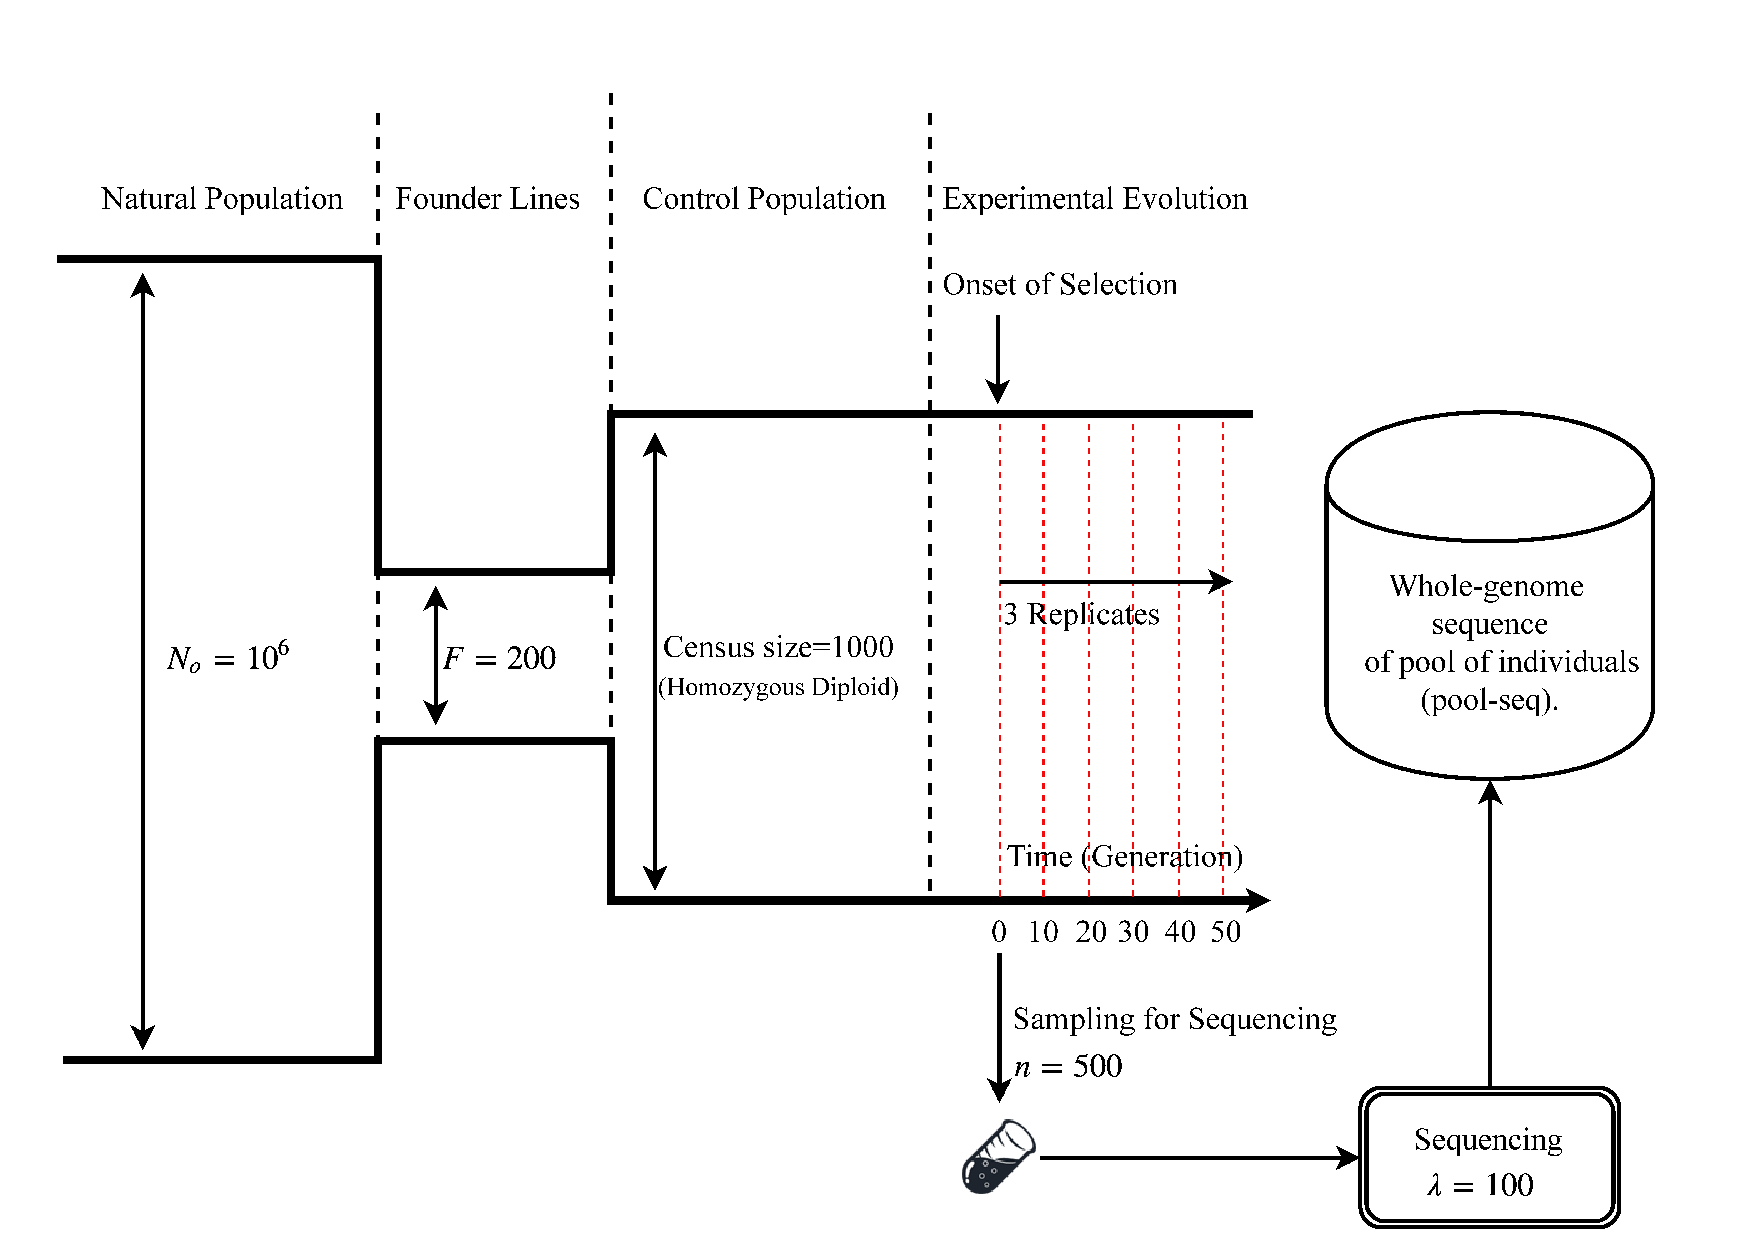
\includegraphics[trim=0in 0in .2in 0.02in , 
	clip,width=0.7\textwidth]{ExperimentalEvolution.eps}\\
	
	\begin{tabular}{l|l}
		\hline\\
		(B) &(C)\\
		\raisebox{0.1in}{
			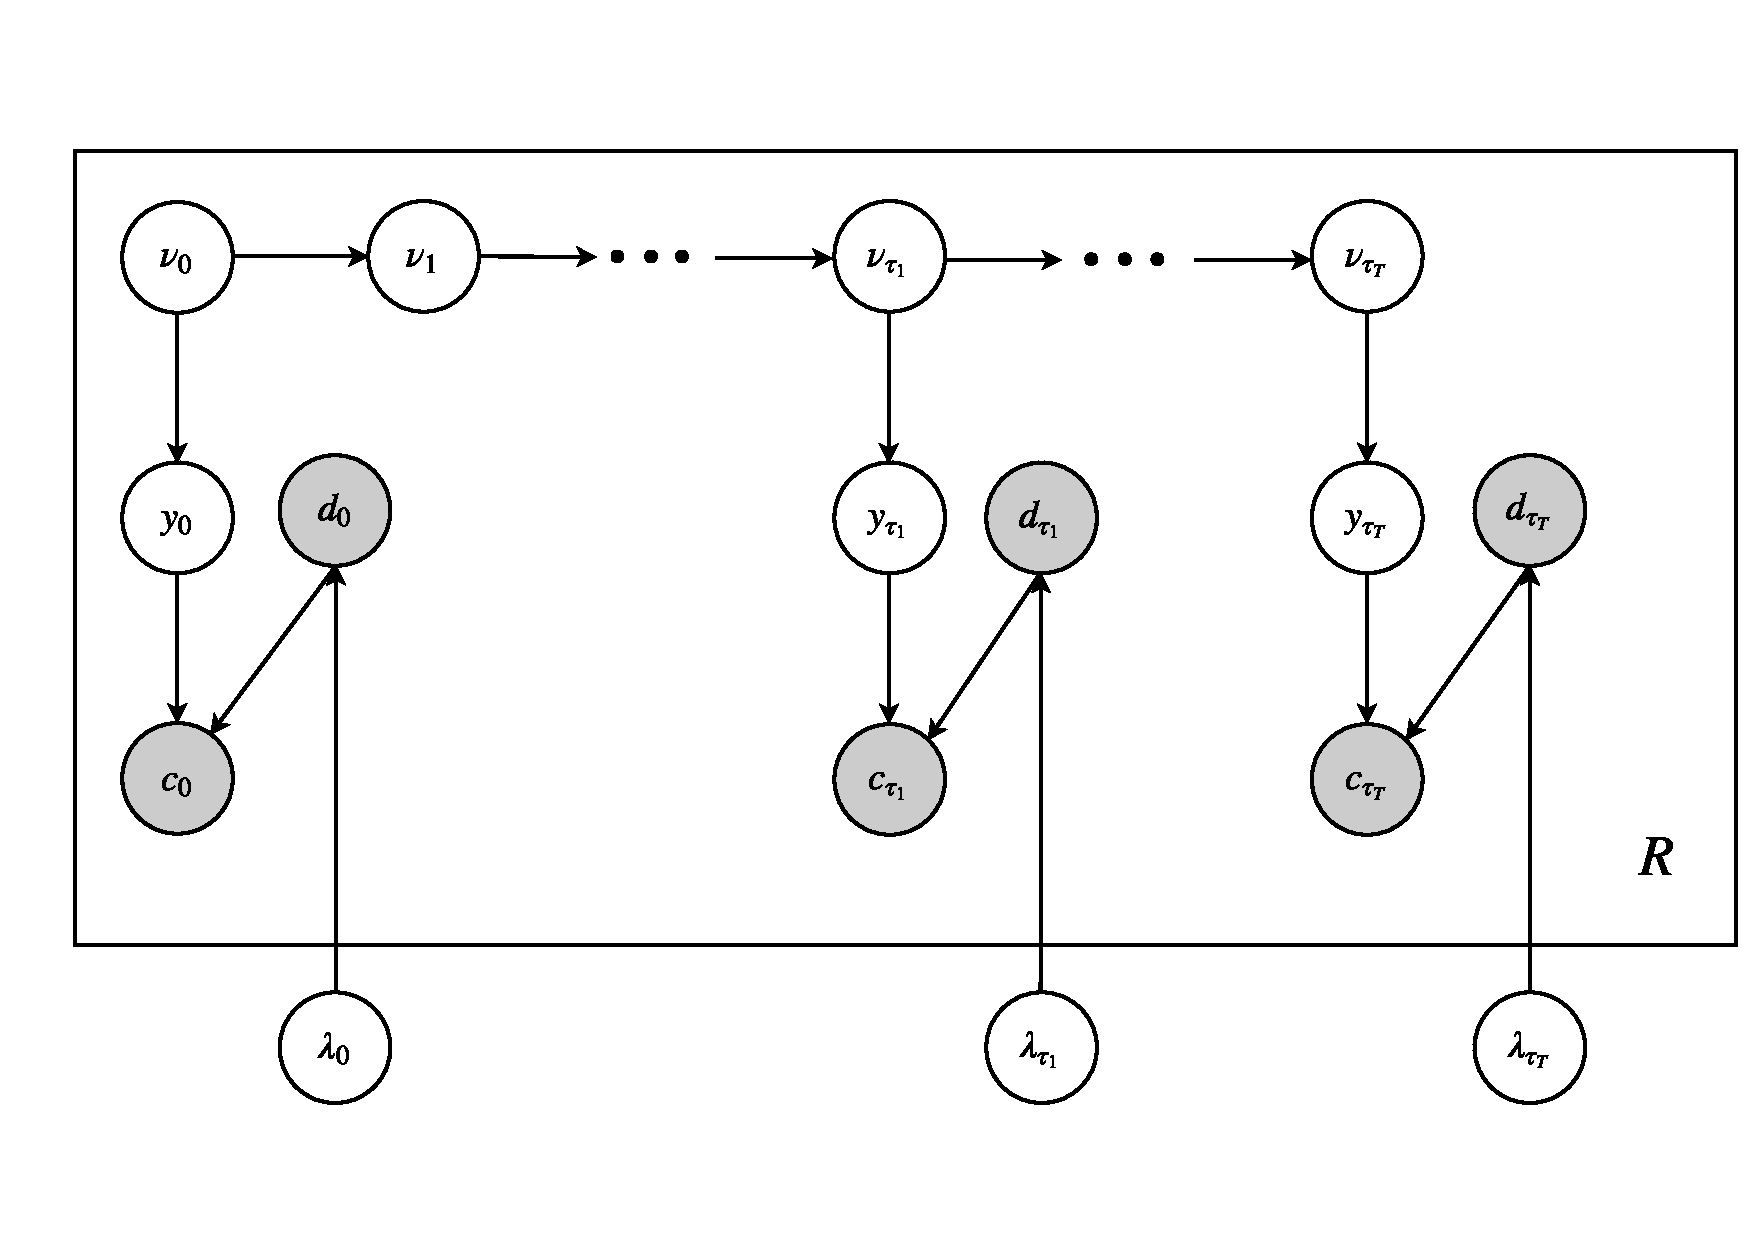
\includegraphics[trim=0in 0.in 0in 
			0.0in,clip,width=0.44\textwidth]{HMMGM.eps}}
		& 	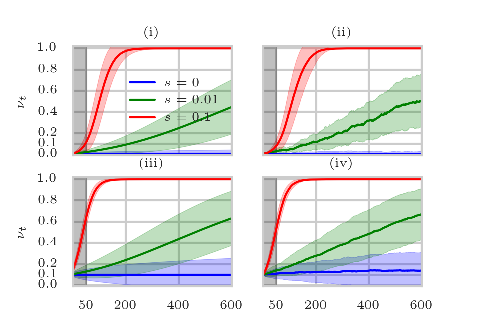
\includegraphics[trim=0in 0.in 0in 
		0.0in,clip,width=0.44\textwidth]{AF.eps}	
		
	\end{tabular}
	\hspace{-1in}
	\caption{{\bf Evolve and Resequence Selection Experiments on \dmel.}
		(A) Typical configuration in which time-series data is 
		collected for
		\dmel. A small set of founder lines ($F=200$) is selected from a
		large population ($N_o=10^{6}$), and used to create a 
		sub-population
		of isofemale lines. Multiple replicates of the population are
		evolved and resequenced to collect time-series genomic data. For
		sequencing, $n$ individuals are randomly sampled and sequenced 
		with
		coverage $\lambda$.  (B) Graphical model showing dependence of 
		the
		random variables in the single-locus model used to compute 
		\comale\
		statistics. Observed variables, $c$ (derived allele read count) 
		and
		$d$ (total read count) are shaded. The variables $\nu,y,\lambda$
		denote allele frequency, sampled allele frequency, and mean
		sequencing coverage, respectively. (C) Mean and 95\% confidence
		interval of the theoretical (i,iii) and empirical (ii,iv)
		trajectories of the favored allele for hard (i,ii) and soft 
		(iii,iv)
		sweep scenarios and $N=1000$.  The first $50$ generations are 
		shaded
		in gray to represent the sampling span of sampling in short-term
		experiments, illustrating the difficulty in predicting 
		selection at
		early stages of selective sweep.  }
	\label{fig:1}
\end{figure*}

\section{Materials and Methods}
\label{sec:method}
Consider a panmictic diploid population with fixed size of $N$
individuals.  Let $\bm{ \nu} =\{\nu_t\}_{t\in\Tc}$ be frequencies of
the derived allele at generations $t\in\Tc$ for a given variant, where
at generations $\Tc= \{\tau_i: 0\le \tau_0<\tau_1\ldots< \tau_T\}$
samples of $n$ individuals are chosen for pooled sequencing. The
experiment is replicated $R$ times. We denote allele frequencies of
the $R$ replicates by the set $\{\bm{\nu}\}_R$.  To identify the genes
and variants that are responding to selection pressure, we use the
following procedure:
\begin{enumerate}
	\item {\bf Estimating population size.} The procedure starts by
	estimating the effective population size, $\hN$, under the
	assumption that much of the genome is evolving neutrally.
	\item {\bf Estimating selection parameters.} For each polymorphic
	site, selection and dominance parameters $s,h$ are estimated so
	as to maximize the likelihood of the time series data, given $\hN$.
	\item {\bf Computing likelihood statistics.} For each variant, a
	log-odds ratio of the likelihood of selection model ($s>0$) to the
	likelihood of neutral evolution/drift model is computed. Likelihood
	ratios in a genomic region are combined to compute the \comale\
	statistic for the region.
	\item {\bf Hypothesis testing.} An empirical null distribution of the
	\comale\ statistic is calculated using genome-wide drift
	simulations, and used to compute $p$-values and thresholds for a
	specified FDR. We perform single locus hypothesis testing within
	selected regions to identify significant variants and report genes
	that intersect with the selected variants.
\end{enumerate}
These steps are described in detail below.
\subsection{Estimating Population Size}
Methods for estimating population sizes from temporal neutral
evolution data have been
developed~\cite{williamson1999using,anderson2000monte,
	bollback2008estimation, Terhorst2015Multi,jonas2016estimating}.
Here, we aim to extend these models to explicitly model the sampling
noise that arise in pool-seq data. Specifically, we model the
variation in sequence coverage over different locations, and the noise
due to sequencing only a subset of the individuals in the population.
In addition, many existing
methods~\cite{bollback2008estimation,feder2014Identifying,topa2015gaussian,Terhorst2015Multi}
are designed for large populations, and model frequency as a
continuous quantity. We observed that using Brownian motion to model
frequency drift may be inadequate for small populations, low starting
frequencies and sparse sampling (in time), factors that are common in
experimental evolution (see Results, \ref{fig:power}A-C, and
\ref{fig:markov}). To this end, we model the Wright-Fisher Markov
process for generating pool-seq data~(\ref{proc:arya}) via a
{discrete} HMM (~\ref{fig:1}-B). We start by computing a likelihood
function for the population size given neutral pool-seq data.


\paragraph{Likelihood for Neutral Model.}
We model the allele frequency counts $2N\nu_t$ as being sampled from a
Binomial distribution. Specifically,
\begin{eqnarray*} 
	\nu_0 &\sim& \pi,\\
	2N\nu_t|\nu_{t-1} &\sim& \bino(2N,\nu_{t-1}) 
\end{eqnarray*}
where $\pi$ is the global distribution of allele frequencies in the
base population. 
Note that  $\pi$  
depends on the
demographic history of the founder lines and can be estimated from site 
frequency spectrum(see~\ref{fig:sfs}) of the initial population. For notational 
convenience, henceforth we omit the dependence of likelihoods to the 
parameter $\pi$.

To estimate frequency after $\tau$ transitions, it is enough to
specify the $2N\times2N$ transition matrix $P^{(\tau)}$, where
$P^{(\tau)}[i,j]$ denotes probability of change in allele frequency
from ${i}/{2N}$ to ${j}/{2N}$ in $\tau$ generations:
\beq
P^{(1)}[i,j] &= \pr\left(\nu_{t+1}=\frac{j}{2N} \left| \right. 
\nu_{t}=\frac{i}{2N}\right)\\
&={2N \choose j} s  \nu_{t}^j
(1-\nu_{t})^{2N-j}, \label{eq:P1}
\eeq
\beq
P^{(\tau)} =   P^{(\tau-1)}P^{(1)} \label{eq:Pt}
\eeq
Furthermore, in an E\&R experiment, $n\le N$ individuals are randomly
selected for sequencing. The {sampled allele frequencies},
$\{y_{t}\}_{t\in\Tc}$, are also Binomially distributed \beq 2ny_{t}
\sim \text{Binomial}(2n,\nu_t) \eeq We introduce the $2N\times2n$
sampling matrix $Y$, where $Y[i,j]$ stores the probability that the
sample allele frequency is ${j}/{2n}$ given that the true allele
frequency is ${i}/{2N}$.


We denote the pool-seq data for that variant as $\{x_t = \langle
c_t,d_t \rangle\}_{t\in\Tc}$ where $d_t, c_t$ represent the coverage,
and the read count of the derived allele, respectively. Let
$\{\lambda_t\}_{t\in\Tc}$ be the sequencing coverage at different
generations. Then, the observed data are sampled according to
\begin{equation} d_t \sim \poiss(\lambda_t), \hspace{1in} c_t \sim
	\bino(d_t,y_t) 
\end{equation}
The emission probability for a observed tuple $x_t=\langle d_t,
c_t\rangle $ is 
\begin{equation} {\bf e}_{i}(x_t) = {d_t \choose c_t}
	\left(\frac{i}{2n} \right)^{c_t}\left (1- \frac{i}{2n}
	\right)^{d_t-c_t} .  
\end{equation}
For $1\le t\le T, 1\le j\le 2N$, let $\alpha_{t,j}$ denote the
probability of emitting $x_1,x_2,\ldots,x_t$ and reaching state $j$ at
$\tau_t$. Then, $\alpha_{t}$ can be computed using the
forward-procedure~\cite{durbin1998biological}:
\begin{align}
	\alpha_t^T&=\alpha_{t-1}^T P^{(\delta_t)}\text{diag}(Y\bfe(x_t))
	\label{eq:hmm}
\end{align}
where $\delta_t=\tau_t-\tau_{t-1}$. The joint likelihood of the
observed data from $R$ independent observations is given by
\beq
\Lc(N|\{\bm{x}\}_R, 
n)&=\prod_{r=1}^R\Lc(N|\bm{x}^{(r)},n)=\pr(\{\bm{x}\}_R|N,n)\\& =	
\prod_{r=1}^R \sum_i\alpha_{T,i}^{(r)}
\label{eq:hmmlik}
\eeq
where $\bm{x}=\{x_t\}_{t\in \Tc}$. The graphical model and the generative 
process for which data is being generated is depicted in~\ref{fig:1}-B 
and~\ref{proc:arya}, respectively.

Finally, the last step is to compute an estimate $\hN$ that maximizes
the likelihood of all $M$ variants in whole genome. Let
$\bm{x}_i^{(r)}$ denote the time-series data of the $i$-th variant in
replicate $r$. Then,
\begin{equation}
	\hN =
	\underset{N}{\arg \max} \prod_{i=1}^M  \prod_{r=1}^R\Lc(N|\bm{x}_i^{(r)})
	\label{eq:mlen}
\end{equation}

\subsection{Estimating Selection Parameters}

\paragraph{Likelihood for Selection Model.}
Assume that the site is evolving under selection constraints $s\in
\Rbb$, $h\in \Rbb_+$, where $s$ and $h$ denote selection strength and 
dominance parameters ,
respectively. By definition, the relative fitness values of genotypes
0$|$0, 0$|$1 and 1$|$1 are given by $w_{00}=1$, $w_{01}=1+hs$ and
$w_{11}=1+s$.  Then, $\nusp$, the frequency at time
$\tau_{t}+1$ (one generation ahead), can be estimated using: 
\beq 
\hat{\nu}_{t^+} =
\mathbb{E}[\nusp|s,h,\nu_t]&=\frac{w_{11}\nu_t^2 +
	w_{01}\nu_t(1-\nu_t)}{w_{11}\nu^2_t + 2w_{01}\nu_t(1-\nu_t) +
	w_{00}(1-\nu_t)^2}\\
&=\nu_t+\frac{s(h+(1-2h)\nu_t)\nu_t(1-\nu_t)}{1+s\nu_t(2h+(1-2h)\nu_t))}.
\label{eq:transition}
\eeq
The machinery for computing likelihood of the selection parameters is 
identical to that of population size, except for transition matrices. Hence, here 
we only describe the definition transition matrix $Q_{s,h}$ of the selection 
model.
Let $Q^{(\tau)}_{s,h}[i,j]$ denote the
probability of transition from ${i}/{2N}$ to ${j}/{2N}$ in
$\tau$ generations, then (See~\cite{Ewens2012Mathematical}, Pg.~24, 
Eqn.~$1.58$-$1.59$):
\beq
Q^{(1)}_{s,h}[i,j] &= \pr\left(\nusp=\frac{j}{2N} \left\lvert
\nu_{t}=\frac{i}{2N};s,h,N \right .\right)\\
&    ={2N \choose j}
\hat{\nu}_{t^+}^{j} (1-\hat{\nu}_{t^+})^{2N-j}\label{eq:Q1}
\eeq
\beq
Q^{(\tau)}_{s,h} &= Q^{(\tau-1)}_{s,h}Q^{(1)}_{s,h}\label{eq:Qt}  
\eeq
The maximum likelihood estimates are given by
\beq
\hs,\hh = \underset{s,h}{\arg \max} \prod_{r=1}^R \Lc(s,h|\bm{x}^{(r)},\hN) 
\label{eq:mlesh}
\eeq

Using grid search, we first estimate $N$ (Eq.~\ref{eq:mlen}), and
subsequently, we estimate parameters $s,h$ 
(Eq.~\ref{eq:mlesh},~\ref{fig:slikes}). By
broadcasting and vectorizing the grid search operations across all
variants, the genome scan on millions of polymorphisms can be done in
significantly smaller time than iterating a numerical optimization
routine for each variant(see Results and \ref{fig:runTime}).
\subsection{Empirical Likelihood Ratio Statistics}
The  likelihood
ratio statistic for testing directional selection, to be computed for each variant, 
is given by
\beq
H &= -2 \log 
\left(\frac{\Lc(\bar{s},0.5|\{\bm{x}\}_R,\hN)}{\Lc(0,0.5|\{\bm{x}\}_R,\hN)}\right),\\
\label{eq:ELRS}
\eeq
where $\bar{s} = \underset{s}{\arg \max} \prod_{r=1}^R 
\Lc(s,0.5|\bm{x}^{(r)},\hN)$. Similarly we can define a test statistic for testing 
if selection is dominant by
\beq
D &= -2 \log 
\left(\frac{\Lc(\hs,\hh|\{\bm{x}\}_R,\hN)}{\Lc(\bar{s},0.5|\{\bm{x}\}_R,\hN)}\right).
\eeq



While extending the single-locus WF model to a multiple linked-loci
can improve the power of the model~\cite{Terhorst2015Multi}, it is
computationally and statistically expensive to compute exact
likelihood. In addition, computing linked-loci joint likelihood requires  
haplotype resolved data, which pool-seq
does not provide. Here, similar to Nielsen~\emph{et
	al}~\cite{nielsen2005genomic}, we calculate \emph{composite likelihood
	ratio} score for a genomic region.
\begin{equation}
	\Hc = \frac{1}{|L|}\sum_{\ell \in L} H_\ell.
	\label{eq:pihmm}
\end{equation}
where $L$ is a collection of segregating sites and $H_\ell$ is the
likelihood ratio score based for each variant $\ell$ in $L$.  The
optimal value of the hyper-parameter $L$ depends upon a number of
factors, including initial frequency of the favored allele,
recombination rates, linkage of the favored allele to neighboring
variants, population size, coverage, and time since the onset of
selection (duration of the experiment). In~\ref{sec:winSize}, we
provide a heuristic to compute a reasonable value of $L$, based on
experimental data. 

We work with a normalized value of $\Hc$, given by
\begin{equation} \Hc_i^*=\frac{\Hc_i-\mu_\Cc}{\sigma_\Cc},
	\hspace{0.5in} \forall i \in \Cc,
\end{equation} 
where $\mu_\Cc$ and $\sigma_\Cc$ are the mean and standard deviation
of $\Hc$ values in a large region $\Cc$. We found different
chromosomes to have different distribution of $\Hc_i$ values, and
therefore decided to use single chromosomes as $\Cc$.
\subsection{Hypothesis Testing}
\paragraph{Single-Locus tests.}
Under neutrality, Log-likelihood ratios can be approximated by $\Xc^2$
distribution~\cite{williams2001weighing}, and $p$-values can be
computed directly. However, Feder \emph{et
	al.}~\cite{feder2014Identifying} showed that when the number of
independent samples (replicates) is small, $\Xc^2$ is a crude
approximation to the true null distribution and results in more false
positive.  Following their suggestion, we first compute the empirical
null distribution using simulations with the estimated population size
(See~\ref{proc:arya}). The empirical null distribution of statistic
$H$ is used to compute $p$-values as the fraction of null values that
exceed the test score.  Finally, we use Storey and Tibshirani's
method~\cite{storey2003statistical} to control for False Discovery
Rate in multiple testing.


\paragraph{Composite likelihood tests.}

Similar to single-locus tests, we compute the null distribution of the
$\Hc^*$ statistic using whole-genome simulations with the estimated
population size, and subsequently compute FDR. The simulations for
generating the null distribution of $\Hc^*$ are described next. 

\subsection{Simulations}\label{sec:sims}
We use the same simulation procedure for two purposes. First, we use
them to test the power of \comale\ against other methods in small
genomic windows. Second, we use the simulations to generate the
distribution of null values for the statistic to compute empirical
$p$-values. We mainly chose parameters that are relevant to \dmel
experimental evolution~\cite{kofler2013guide}. See also \ref{fig:1}-A
for illustration. 
\begin{enumerate}
	\item {\bf Creating initial founder line haplotypes.} Using
	\texttt{msms}~\cite{ewing2010msms}, we created neutral populations
	for $F$ founding haplotypes with command \texttt{\$./msms <F> 1 -t
		<2$\mu WN_o$> -r <$2rWN_o$> <W>}, where $F=200$ is number of 
	founder
	lines, $N_o=10^6$ is effective founder population size,
	$r=2\times10^{-8}$ is recombination rate, $\mu=2\times 10^{-9}$ is
	mutation rate. The window size $W$ is used to compute $\theta=2\mu
	N_oW$ and $\rho=2N_orW$. We chose $W=50$Kbp for simulating
	individual windows for performance evaluations, and $W=20$Mbp for
	simulating \dmel chromosomes for $p$-value computations.
	
	\item{\bf Creating initial diploid population.} An initial set of
	$F=200$ haplotypes was created from step I, and duplicated to create
	$F$ homozygous diploid individuals to simulate generation of inbred
	lines. $N$ diploid individuals were generated by sampling with
	replacement from the $F$ individuals.
	
	\item{\bf Forward Simulation.} We used forward simulations for
	evolving populations under selection. We also consider selection
	regimes which the favored allele is chosen from standing variation
	(not \emph{de novo} mutations). Given initial diploid population,
	position of the site under selection, selection strength $s$, number
	of replicates $R=3$, recombination rate $r=2\times10^{-8}$ and
	sampling times $\Tc=\{0,10,20,30,40,50\}$,
	\texttt{simuPop}~\cite{peng2005simupop} was used to perform forward
	simulation and compute allele frequencies for all of the $R$
	replicates.  For hard sweep (respectively, soft sweep) simulations
	we randomly chose a site with initial frequency of $\nu_0=0.005$
	(respectively, $\nu_0=0.1$) to be the favored allele. For generating
	the null distribution with drift for $p$-value computations, we used
	this procedure with $s=0$.
	
	\item{\bf Sequencing Simulation.} Given allele frequency trajectories
	we sampled depth of each site in each replicate identically and
	independently from Poisson($\lambda$), where $\lambda \in
	\{30,100,300\}$ is the coverage for the experiment. Once depth $d$
	is drawn for the site with frequency $\nu$, the number of reads $c$
	carrying the derived allele are sampled according to
	Binomial$(d,\nu)$. For experiments with finite depth the tuple
	$\langle c,d\rangle$ is the input data for each site.
\end{enumerate}

\section{Results}
\paragraph{Modeling Allele Frequency Trajectories in Small Populations.} 
We first tested the goodness of fit of the discrete versus Brownian motion (a 
continuous-state model) in modeling allele frequency trajectories, under 
general E\&R
parameters.  For this purpose, we conducted $100$K simulations with
two time samples $\Tc=\{0,\tau\}$ where $\tau\in \{1,10,100\}$ is the
parameter controlling the density of sampling in time.  In addition,
we repeated simulations for different values of starting frequency
$\nu_0\in\{0.005,0.1\}$ (i.e., hard and soft sweep) and selection
strength $s\in\{0,0.1\}$ (i.e., neutral and selection). Then, given
initial frequency $\nu_0$, we computed the expected distribution of
the frequency of the next sample $\nu_\tau$ under two models to make a
comparison.  \ref{fig:markov}A-F shows that Brownian motion
(continuous model) is inadequate when $\nu_0$ is far from $0.5$, or
when sampling times are sparse ($\tau>1$). If the favored allele
arises from standing variation in a neutral population, it is unlikely
to have frequency close to $0.5$, and the starting frequencies are
usually much smaller (see \ref{fig:sfs}). Moreover, in typical \dmel
experiments for example, sampling is sparse. Often, the experiment is
designed so that $10\le\tau\le100$~\cite{kofler2013guide,
	orozco2012adaptation, zhou2011experimental,franssen2015patterns}.

% XXX Not sufficient to say 'in contrast to brownian motion, markov...
% Please check the rewrite of this part
In contrast to the Brownian motion approximation, discrete Markov
chain predictions (Eq.~\ref{eq:Qt}) are highly consistent with
empirical data for a wide range of simulation parameters
(\ref{fig:markov}A-M). Moreover, the discrete markov chain can be
modified to model the case when the the allele is under
selection. 

\begin{figure*}
	\centering
	\includegraphics[width=\textwidth]{{markovDists}.eps}
	\caption{{\bf Comparison of empirical distributions of allele
			frequencies (red) versus predictions from Brownian
			Motion (green), and Markov chain (blue).}\\
		Comparison of empirical and theoretical distributions under
		neutral evolution (panels A-F) and selection (panels G-M)
		with different starting frequencies $\nu_0\in\{0.005,0.1\}$
		and sampling times of $\Tc=\{0,\tau\}$, where $\tau \in
		\{1,10,100\}$ and $N=1000	$.  For each panel, the empirical 
		distribution
		was computed over 100,000 simulations.  Brownian motion
		(Gaussian approximation) provides poor approximations when
		initial frequency is far from 0.5 (A) or sampling is sparse
		(B,C,E,F). In addition, Brownian motion can only provide
		approximations under neutral evolution. In contrast, Markov
		chain consistently provides a good approximation in all
		cases.}
	\label{fig:markov}
\end{figure*}

\paragraph{Detection Power.} 
We compared the performance of \comale\ against other methods for
detecting selection. For each method we calculated detection power as
the percentage of true-positives identified with false-positive rate
$\le 0.05$. For each configuration (specified with values for
selection coefficient $s$, starting allele frequency $\nu_0$ and
coverage $\lambda$), power of each method is evaluated over $2000$
distinct simulations, half of which modeled neutral evolution and the
rest modeled positive selection.



We compared the power of \comale\ with Gaussian process
(GP)~\cite{Terhorst2015Multi}, FIT~\cite{feder2014Identifying}, and
CMH~\cite{agresti2011categorical} statistics.  FIT and GP convert read
counts to allele frequencies prior to computing the test statistic.
\comale\ shows the highest power in all cases and the power stays
relatively high even for low coverage (\ref{fig:power} and
\ref{tab:power}). In particular, the difference in performance of
\comale\ with other methods is pronounced when starting frequency is
low.  The advantage of \comale\ stems from the fact that favored
allele with low starting frequency might be missed by low coverage
sequencing. In this case, incorporating the signal from linked sites
becomes increasingly important. We note that methods using only two
time points, such as CMH, do relatively well for high selection values
and high coverage. However, the use of time-series data can increase
detection power in low coverage experiments or when starting frequency
is low. Moreover, time-series data provide means for estimating
selection parameters $s,h$ (see below). Finally, as \comale\ is robust
to change of coverage, our results (\ref{fig:power}B,C) suggest that
taking many samples with lower coverage is preferable to sparse
sampling with higher coverage. For comparison purposes, we also tested
\comale\ using the single locus statistic ($L=1$). For the most part,
\comale\ showed an improvement over other methods even with $L=1$, or
showed similar performance. The performance improved with higher $L$.


\begin{figure*}
	\centering
	\includegraphics[width=\textwidth]{power.eps}
	\caption{ {\bf Power calculations for detection of selection.}\\
		Detection power for \comale ($\Hc$), Frequency Increment
		Test (FIT), Gaussian Process (GP), and CMH under hard (A-C)
		and soft sweep (D-F) scenarios. $\lambda$, $s$ denote the
		mean coverage and selection coefficient, respectively.
		Orange hexagons represent the performance of \comale\ when
		the maximum of the single-locus statistic is used to make a
		decision for the genomic region, while the red circle
		corresponds to the performance of \comale\ when single locus
		statistics are averaged over the region.  The $y$-axis
		measures power -- sensitivity with false positive rate FPR
		$\le 0.05$ -- for $2,000$ simulations with $N=1,000$,
		$L=50$Kbp. The horizontal line reflects the power of a
		random classifier.  In all simulations, 3 replicates are
		evolved and sampled at generations
		$\Tc=\{0,10,20,30,40,50\}$.}
	\label{fig:power}
\end{figure*}
\paragraph{Site-identification.}
In general, localizing the favored variant, using pool-seq data is a
nontrivial task due to extensive linkage
disequilibrium~\cite{tobler2014massive}.  To measure performance, we
sorted variants by their $H$ scores and computed rank of the favored
allele for each method. For each setting of $\nu_0$ and $s$, we
conducted $1000$ simulations and computed the rank of the favored
mutation in each simulation. The cumulative distribution of the rank
of the favored allele in 1000 simulation for each setting
(\ref{fig:rank}) shows that \comale\ outperforms other statistics.

An interesting observation is revisiting the contrast between
site-identification and
detection~\cite{long2013massive,tobler2014massive}.  When selection
strength is high, detection is easier (\ref{fig:power}A-F), but
site-identification is harder, due to the high LD between flanking
variants and the favored allele (\ref{fig:rank}A-F).  Moreover,
site-identification becomes more difficult whenever the initial
frequency of the favored allele is low, i.e., at the onset of
selection, LD between favored allele and its nearby variants is
high. For example, when coverage $\lambda=100$ and selection
coefficient $s=0.1$, the detection power is 75\% for hard sweep, but
100\% for soft sweep (\ref{fig:power}B-E). In contrast, the favored
site was ranked as the top in 14\% of hard sweep cases, compared to
and 95\% of soft sweep simulations. 


\begin{figure*}
	\centering
	\includegraphics[trim=.2in 0 .2in 0, 
	clip,width=\textwidth]{{rank100.0}.eps}
	\caption{{\bf Ranking performance for 100$\times$ coverage.}\\
		Cumulative Distribution Function (CDF) of the distribution
		of the rank of the favored allele in 1000 simulations for
		\comale\ ($H$), Gaussian Process (GP), CMH, and Frequency
		Increment Test (FIT), for different values of selection
		coefficient $s$ and initial carrier frequency. Note that the
		individual variant \comale\ score ($H$) is used to rank
		variants.  The Area Under Curve (AUC) is computed as an overall
		quantitative measure to compare the performance of methods
		for each configuration. In all simulations, 3 replicates with $N=1000$ 
		are evolved and 
		sampled at generations 
		$\Tc=\{0,10,20,30,40,50\}$.}
	\label{fig:rank}
\end{figure*}


\paragraph{Estimating Parameters.}
\comale\ estimates effective population size $\hN$ and selection
parameters, $\hat{s}$ and $\hat{h}$, as a byproduct of the hypothesis
testing. We computed bias of selection fitness ($s-\hat{s}$) and
dominance ($h-\hat{h}$) for of \comale\ and GP for 1000 simulations in
each setting. The distribution of the error (bias) for 100$\times$
coverage is presented in \ref{fig:bias100} for different
configurations.  \ref{fig:bias30} and \ref{fig:biasinf} provide the
distribution of estimation errors for 30$\times$, and 300$\times$
coverage, respectively.  For hard sweep, \comale\ provides estimates
of $s$ with lower variance of bias (\ref{fig:bias100}A and
\ref{fig:biasNull}). In soft sweep, GP and \comale\ both provide unbiased
estimates of $s$ with low variance
(\ref{fig:bias100}B). \ref{fig:bias100}~C-D shows that \comale\
provides unbiased estimates of $h$ as well when $h\in\{0,0.5,1,2\}$
and $s=0.1$.  We also tested if \comale\ provide unbiased estimates of
$N$, by estimating population size on 1000 simulations when $N\in
\{200,600,1000\}$. As shown in~\ref{fig:estimateNMLE}-A 
and~\ref{fig:estimateN}A-C, maximum
likelihood is attained at true value of the parameter.


\begin{figure*}
	\centering
	\includegraphics[width=0.7\textwidth]{{bias.100}.eps}
	\caption{{\bf Distribution of bias for 100$\times$ coverage.}\\ The
		distribution of bias ($s-\hat{s}$) in estimating selection
		coefficient over 1000 simulations using Gaussian Process (GP) and
		\comale\ ($H$) is shown for a range of choices for the selection
		coefficient $s$ and starting carrier frequency $\nu_0$, when
		coverage $\lambda=100$ (Panels A,B). GP and \comale\ have similar
		variance in estimates of $s$ for soft sweep, while \comale\ provides
		lower variance in hard sweep. Also see \ref{tab:biasdist}. Panels C,D
		show the variance in the estimation of $h$. 
		In all simulations, 3 replicates are evolved and sampled at generations 
		$\Tc=\{0,10,20,30,40,50\}$.}
	\label{fig:bias100}
\end{figure*}

\paragraph{Running Time.}
As \comale\ does not compute exact likelihood of a region (i.e., does
not explicitly model linkage between sites), the complexity of
scanning a genome is linear in number of polymorphisms.  Calculating
score of each variant requires and $\Oc(TRN^3)$ computation
for $\Hc$. However, most of the operations
are can be vectorized for all replicates to make the effective running
time for each variant.  We
conducted $1000$ simulations and measured running times for computing 
site 
statistics $H$, FIT, CMH and GP with different number of linked-loci.  Our
analysis reveals (\ref{fig:runTime}) that \comale\ is orders of
magnitude faster than GP, and comparable to FIT. While slower than CMH
on the time per variant, the actual running times are comparable after
vectorization and broadcasting over variants (see below).

These times can have a practical consequence. For instance, to run GP
in the single locus mode on the entire pool-seq data of the \dmel genome 
from a
small sample ($\approx$1.6M variant sites), it would take 1444 CPU-hours
($\approx$ 1 CPU-month). In contrast, after vectorizing and
broadcasting operations for all variants operations using
\texttt{numba} package, \comale\ took 75 minutes to perform an
scan, including precomputation, while the fastest method, CMH, took 17 
minutes.

\begin{figure*}
	\centering
	\includegraphics[width=0.75\textwidth]{{runTime.eps}}
	\caption{{\bf Running time.}\\ Box plots of running time per
		variant (CPU-secs.) of \comale ($\Hc$), CMH, FIT, and
		GP with single, 3, 5, 7, and 10 loci over 1000 simulations
		conducted on a workstation with Intel Core i7
		processor. The average running time for each method is shown
		on the x-axis.
		In all simulations, 3 replicates are evolved and sampled at generations 
		$\Tc=\{0,10,20,30,40,50\}$.}
	\label{fig:runTime}
\end{figure*}


\subsection{Analysis of a \dmel Adaptation to Alternating 
	Temperatures}\label{sec:dmel}
We applied \comale\ to the 
\datadm~\cite{orozco2012adaptation,franssen2015patterns}, where
3 replicate samples were chosen from a population of \dmel for 59
generations under alternating 12-hour cycles of  hot stressful (28$^{\circ}$C)
and non-stressful (18$^{\circ}$C) temperatures and sequenced.  In this 
dataset,
sequencing coverage is different across replicates and generations
(see S2 Fig of~\cite{Terhorst2015Multi}) which makes variant depths
highly heterogeneous (\ref{fig:depthHetero}). 

We first filtered out heterochromatic, centromeric and telomeric
regions~\cite{fiston2010drosophila}, and those variants that have
collective coverage of more that 1500 in all 13 populations: three
replicates at the base population, two replicates at generation 15,
one replicate at generation 23, one replicate at generation 27, three
replicates at generation 37 and three replicates at generation
59. After filtering, we ended up with 1,605,714 variants.

Next, we estimated genome-wide population size $\hN=250$
(\ref{fig:estimateNMLE}-B and \ref{fig:estimateN}-E) which is consistent with 
previous
studies~\cite{orozco2012adaptation,jonas2016estimating}. The
likelihood curves of \comale\ are sharper around the optimum compared
to that of Bollback et. al~\cite{bollback2008estimation}'s method (see
Supplementary Fig. 1 in~\cite{orozco2012adaptation}).  Also,
chromosomes 3L and 3R appear to have smaller population
size, $\hN=200,150$, respectively. 
Others have
made similar observations on this data. In particular,
J\'{o}n\'{a}s~\emph{et al.}~\cite{jonas2016estimating} shown that the 
chromosome-wise population
size varies even more when it is computed for each replicate
separately (see Table 1 in~\cite{jonas2016estimating}). For instance,
$\hN$ is 131 for chromosome 3R replicate 1, while it is 328 for chromosome 
X 
replicate 2.  

\begin{figure*}
	\centering
	\includegraphics[width=\textwidth]{estimateNMLE.eps}
	\caption{{\bf Estimating population size.}  (A) Distribution
		of bias in estimating $N$, computed on 1000 neutral
		simulations for each $N\in\{200,600,1000\}$ when $W=10$Mbp and 
		$r=2\times10^{-8}$. (B) 
		Estimates
		of population size for \datadm. For each case, the
		distribution of estimator is computed by 100 bootstrap
		computations using 1000 variants each. The multiple modes
		are an artifact of grid search used to speed up
		computation. (C) Distribution of the population 	size
		estimates on the yeast dataset.  Despite large census
		population size ($10^6-10^7$~\cite{burke2014standing}), this
		dataset exhibits much smaller effective population size
		($\hN=2000$). }
	\label{fig:estimateNMLE}
\end{figure*}

While it would be ideal to compute \comale\ statistic for each
replicate and chromosome separately, computing empirical $p$-values
and significant regions become computationally intensive as empirical
null distribution of each replicate and each chromosome needs to be
computed.  Hence, we use a single genome-wide estimate $\hN=250$ in
all analyses, but we normalize statistic $\Hc^*$ separately for each
chromosome.

We use a heuristic calculation (See~\ref{sec:winSize}) to choose the
sliding window size $L$ as the distance where the LD between the
favored mutation and a site $L/2$bp away remains strong. For \dmel
parameters, we obtained $L=30$Kbp. We computed the normalized test
statistic $\Hc^*$ on sliding windows of size of 30Kbp and step size of
5Kbp over the genome (See~\ref{fig:man-dmel-region}-A).

Empirical null distribution of $\Hc^*$ was estimated by creating 100
whole genome simulations (400K statistic values) as described in
Section~\ref{sec:sims}. Then, $p$-value of the test statistic in each
region in the experimental data was calculated as the fraction of the
null statistic values that are greater than or equal to the test
statistic(see~\ref{fig:null-alt}).  After correcting for multiple
testing, we identified $5$ contiguous
intervals~(\ref{fig:man-dmel-region}) satisfying FDR$\le0.05$, and
covering $2,829$ polymorphic sites. We further performed single-locus
hypothesis testing on the $2,829$ sites to identify $174$ individual
variants with FDR $\le0.01$~(\ref{fig:man-dmel-region}-B).

The final set of 174 variants fall within 32 genes(\ref{tab:genes})
including many Serine inhibitory proteases (serpins), and other genes
involved in endocytosis. Recycling of synaptic vesicles is seen to be
blocked at high temperature in temperature sensitive Drosophila
mutants~\cite{kosaka1983reversible}. This is also supported by GO
enrichment analysis, where a single GO term `inhibition of
proteolysis' is found to enriched (corrected $p$-value:0.0041).  To
test for dominant selection, we computed $D$ statistic on simulated
neutral and experimental data, and computed $p$-values accordingly.
After correcting for multiple testing, 96 variants were discovered
with FDR$\le 0.01$~(\ref{fig:man-dmel-snp}). 


\subsection{Analysis of Outcrossing Yeast Populations}
We also applied \comale\ to  $12$ replicate samples of
outcrossing yeast populations~\cite{burke2014standing}, where samples are 
taken at
generations $\Tc=\{0,180,360,540\}$. We observed a significant
variation in the genome-wide site frequency spectrum of certain
populations over different time points for some
replicates~(\ref{fig:yeast-sfs}). The variation does not have an
easily identifiable cause. Therefore, we focused analysis on seven
replicates $r\in\{3,7,8,9,10,11,12\}$ with genome-wide site-frequency
spectrum over the time range~(\ref{fig:yeast-pca}).

We estimated population size to be $\hN=2000$ haplotypes 
(\ref{fig:estimateNMLE}-C and \ref{fig:estimateN}-F), and computed
$\hs$, $\hh$ and $H$ statistic accordingly. To compute $p$-values, we
created 1M single-locus neutral simulations according to experimental
data's initial frequency and coverage. By setting FDR cutoff to
$0.05$, only 18 and 16 variants show significant signal for
directional and dominant selection,
respectively~(\ref{fig:man-dmel-snp}).  Selected variants for
directional selection are clustered in two regions, which match $2$ of
the $5$ regions (regions C and E in Fig. 2-a
in~\cite{burke2014standing}) identified by Burke~\emph{et al.} in
their preliminary analysis. 

\begin{figure*}
	\centering
	\begin{tabular}{c}
		(A)\\
		\includegraphics[trim=0.4in 0.in 0.6in 
		0in,clip,width=0.9\textwidth]{man-dmel-region.eps}\\		
		(B)\\	
		\includegraphics[trim=0.3in 0.in 0.6in 
		.0in,clip,width=0.9\textwidth]{{topVariants.dmel.dir}.eps}
	\end{tabular}
	\caption{{\bf Scan of \comale\ statistic on \datadm.}
		(A)         Manhattan plot of scan for $\Hc^*$ statistic using sliding 
		window of 
		size $L=3000$ over the
		genome.  The dashed line represents cutoff for genome-wide
		FDR$\le0.05$, and identifies 5 contiguous intervals, I1-I5, 
		which are shaded in blue. (B) Trajectories of the selected 
		variants within 
		intervals I1-I5.}
	\label{fig:man-dmel-region}
\end{figure*}



\begin{figure*}
	\centering
	\begin{tabular}{cc}
		\includegraphics[trim=0.4in 0.in 0.6in 
		0.0in,clip,width=0.65\textwidth]{man-yeast-snp.eps}&	
		\raisebox{0.2in}{
			\includegraphics[trim=0in 0.in 0in 
			0.0in,clip,width=0.35\textwidth]{{topVariants.yeast}.eps}}
	\end{tabular}
	\caption{{\bf Single locus analysis of the yeast outcrossing 
			populations.}\\ Manhattan plot 
		of scan single locus \comale\ statistic ($L=1$) for testing directional 
		selection (A) and dominant 
		selection 
		(C).
		The dashed line represents cutoff for  genome-wide FDR$\le0.05$.
		Trajectories of the selected variants are depicted in panels (B) and 
		(D).}
	\label{fig:man-yeast-snp}
\end{figure*}





\section{Discussion}
We developed a computational tool, \comale, that can detect regions
and variants under selection E\&R experiments. Using extensive simulations, 
we show that \comale\
outperforms existing methods in detecting selection, locating the
favored allele, and estimating model parameters.  Also, while
being computationally efficient, \comale\ provide means for estimating
populations size and hypothesis testing.

Many factors such as small population size, finite coverage, linkage
disequilibrium, finite sampling for sequencing, duration of the
experiment and the small number of replicates can limit the power of
tools for analyzing E\&R.  Here, by an discrete modeling, \comale\
estimates population size, and provides unbiased estimates of
$s,h$. It adjusts for heterogeneous coverage of pool-seq data, and
exploits presence of linkage within a region to compute composite
likelihood ratio statistic.


It should be noted that, even though we described \comale\ for small
fixed-size populations, the statistic can be adjusted for other
scenarios, including changing population sizes when the demography is
known. For large populations, transitions can be computed on sparse
data structures, as for large $N$ the transition matrices become
increasingly sparse. Alternatively, frequencies can be binned to
reduce dimensionality.


The comparison of hard and soft sweep scenarios showed that initial
frequency of the favored allele can have an nontrivial effect on the
statistical power for identifying selection. Interestingly, while it
is easier to detect a region undergoing strong selection, it is harder
to locate the favored allele in that region.


There are many directions to improve the analyses presented here.  In
particular, we plan to focus our attention on other organisms with
more complex life cycles, experiments with variable population size
and longer sampling-time-spans. As evolve and resequencing experiments
continue to grow, deeper insights into adaptation will go hand in hand
with improved computational analysis.


\paragraph{Software and Data Availability.}

The source code and running scripts for \comale\ are publicly available at 
\url{https://github.com/airanmehr/clear}. 

\dmel data originally published 
\cite{orozco2012adaptation,franssen2015patterns}. The dataset of the 
\dmel study, until generation 37, is obtained from Dryad 
digital repository (\url{http://datadryad.org}) under 
accession DOI: 
\href{http://datadryad.org/resource/doi:10.5061/dryad.60k68}{10.5061/dryad.60k68}.
Generation 59 of the \dmel study is accessed from
European Sequence Read Archive 
(\href{http://www.ebi.ac.uk/ena/}{http://www.ebi.ac.uk/ena/})  under 
the 
project accession number: PRJEB6340.
The dataset containing experimental evolution of Yeast 
populations~\cite{burke2014standing} is 
downloaded from 
\url{http://wfitch.bio.uci.edu/~tdlong/PapersRawData/BurkeYeast.gz}
%{http://wfitch.bio.uci.edu/~tdlong/PapersRawData/BurkeYeast.gz}
(last accessed 01/24/2017). 
UCSC browser tracks for \dmel and Yeast data analysis are found in Suppl. 
Data 
1 and 2, respectively.
\section*{Acknowledgments}
AI, AA, and VB were supported by grants from the NIH (1R01GM114362) and
NSF (DBI-1458557 and IIS-1318386). CS is supported by the European 
Research 
Council grant ArchAdapt.
The authors also thank the anonymous reviewers whose comments 
substantially improved quality and clarity of this manuscript.

\section*{Conflict of interest}
VB is a co-founder, has an equity interest, and receives income from
Digital Proteomics, LLC (DP).  The terms of this arrangement have been
reviewed and approved by the University of California, San Diego in
accordance with its conflict of interest policies.  DP was not
involved in the research presented here.
\bibliography{library}

\end{document}